\documentclass[12pt, a4paper]{article}

% ==========================================
% 1. KHAI BÁO GÓI THƯ VIỆN (PACKAGES)
% ==========================================
% Bảng mã & Font chữ
\usepackage[utf8]{inputenc}
\usepackage[T5]{fontenc}

% Toán học
\usepackage{amsmath, amssymb}

% Căn lề & Bố cục trang
\usepackage[top=2.2cm, bottom=1.5cm, left=1cm, right=1cm, headheight=15pt]{geometry}
\usepackage{fancyhdr}
\usepackage{needspace}
\usepackage{tkz-tab}

% Đồ họa & Màu sắc
\usepackage{xcolor}
\usepackage{graphicx} 
\usepackage{tikz}
\usetikzlibrary{calc, shapes.geometric, positioning}


% Bảng biểu & Danh sách
\usepackage{colortbl}
\usepackage{array}
\usepackage{makecell}
\usepackage{multirow}
\usepackage{tasks}

% Biểu tượng
\usepackage{fontawesome5}

% ==========================================
% 2. THIẾT LẬP MÀU SẮC CHỦ ĐẠO
% ==========================================
\definecolor{goldyellow}{RGB}{255, 179, 0}
\definecolor{amberorange}{RGB}{230, 115, 0}
\definecolor{lightamber}{RGB}{255, 248, 225}
\definecolor{deepblue}{RGB}{25, 42, 86}
\definecolor{accentred}{RGB}{232, 65, 24}
\definecolor{softgray}{RGB}{220, 220, 222} 
\definecolor{fbblue}{RGB}{15, 80, 200}


% ==========================================
% 3. CẤU HÌNH HEADER & FOOTER
% ==========================================
\pagestyle{fancy}
\fancyhf{}
\renewcommand{\headrulewidth}{0pt}

% Khai báo biến lưu trữ nội dung góc phải của Header
\newcommand{\HeaderRightText}{}

% --- Header ---
\fancyhead[C]{
    \begin{tikzpicture}[remember picture, overlay]
        
        % Dải màu trang trí góc trên
        \path[fill=deepblue] (current page.north west) -- (current page.north east) 
            -- ($(current page.north east) + (0, -1.6cm)$) 
            .. controls ($(current page.north) + (3, -2.0cm)$) and ($(current page.north) + (-3, -0.4cm)$) .. 
            ($(current page.north west) + (0, -1.0cm)$) -- cycle;
            
        \path[fill=goldyellow] (current page.north west) -- (current page.north east) 
            -- ($(current page.north east) + (0, -1.0cm)$) 
            .. controls ($(current page.north) + (4, -1.0cm)$) and ($(current page.north) + (-2, -2.2cm)$) .. 
            ($(current page.north west) + (0, -1.6cm)$) -- cycle;
            
        \path[fill=amberorange] (current page.north west) -- ($(current page.north west) + (6.5cm, 0)$) 
            .. controls ($(current page.north west) + (4.5cm, -1.2cm)$) and ($(current page.north west) + (2cm, -2.0cm)$) .. 
            ($(current page.north west) + (0, -2.0cm)$) -- cycle;
            
        % Logo góc trái Header
        \node[anchor=west, inner sep=0pt] 
            at ($(current page.north west) + (0cm, -0.8cm)$) {
\includegraphics[height=2.0cm]{../../../image/logo-header.png}};
            
        % Text góc phải Header (Tự động lấy từ đối số thứ 3 của \titlebox)
        \node[anchor=east, text=white, font=\small\bfseries\sffamily] 
            at ($(current page.north east) + (-0.8cm, -0.5cm)$) {\HeaderRightText};
    \end{tikzpicture}
}

% --- Footer ---
\fancyfoot[C]{
    \begin{tikzpicture}[remember picture, overlay]
        % Đường kẻ ngang
        \draw[amberorange, line width=1.5pt] 
            ($(current page.south west) + (0cm, 0.4cm)$) -- ($(current page.south east) + (0cm, 0.4cm)$);

        % Dải cong góc phải
        \path[fill=goldyellow] (current page.south east) -- ($(current page.south east) + (-5cm, 0)$) 
            .. controls ($(current page.south east) + (-3cm, 0.8cm)$) and ($(current page.south east) + (-1.5cm, 1.2cm)$) .. 
            ($(current page.south east) + (0, 1.2cm)$) -- cycle;

        % Mạng xã hội
        \node[anchor=west, inner sep=0pt] at ($(current page.south west) + (1cm, 0.8cm)$) {
            \small\sffamily
            \textcolor{fbblue}{\faFacebook\hskip 4pt Toán Anh Huy MATH-STER}
            \hskip 18pt
            \textcolor{black}{\faTiktok\hskip 4pt huymathster}
        };

        % Số trang
        \node[circle, fill=white, draw=amberorange, line width=1.5pt, text=deepblue, font=\large\bfseries\sffamily, inner sep=4pt, minimum size=0.8cm] 
            at ($(current page.south east) + (-1.2cm, 0.6cm)$) {\thepage};
    \end{tikzpicture}
}

% ==========================================
% 4. ĐỊNH NGHĨA MACRO: KHUNG TIÊU ĐỀ
% ==========================================
\newcommand{\titlebox}[3]{
    % Gán nội dung đối số #3 vào biến HeaderRightText
    \gdef\HeaderRightText{#3}
    
    \begin{center}
    \vspace*{-0.5cm}
    \begin{tikzpicture}
        % Khung vô hình (Phantom Box) định chuẩn kích thước
        \node[text width=16cm, inner xsep=0pt, inner ysep=16pt, opacity=0] (MainBox) {
            \begin{minipage}[c]{4.2cm}
                \centering\vspace{0.1cm}
                \rule{2.2cm}{2.2cm} 
                \vspace{0.1cm}
            \end{minipage}%
            \begin{minipage}[c]{11.5cm}
                \centering\vspace{0.15cm}
                {\huge\bfseries\sffamily #2 \par}
                \vspace{0.15cm} 
            \end{minipage}
        };
        
        % Đổ bóng & Nền
        \fill[goldyellow, rounded corners=8pt] ([xshift=5pt, yshift=-5pt]MainBox.south west) rectangle ([xshift=5pt, yshift=-5pt]MainBox.north east);
        \fill[white, rounded corners=8pt] (MainBox.south west) rectangle (MainBox.north east);
        
        % Lưới ô ly & Nền Logo
        \begin{scope}
            \clip[rounded corners=8pt] (MainBox.south west) rectangle (MainBox.north east);
            \draw[step=0.4cm, softgray!50, line width=0.6pt] (MainBox.south west) grid (MainBox.north east);
            \fill[lightamber!60] (MainBox.south west) rectangle ([xshift=4.2cm]MainBox.north west);
        \end{scope}

        % Viền ngoài
        \draw[deepblue, line width=1.5pt, rounded corners=8pt] (MainBox.south west) rectangle (MainBox.north east);

        % Nội dung Text (Lớp trên cùng)
        \node[text width=16cm, inner xsep=0pt, inner ysep=16pt] at (MainBox.center) {
            \begin{minipage}[c]{4.2cm}
                \centering
                % --- ĐIỀU CHỈNH TỌA ĐỘ LOGO Ở ĐÂY ---
                \hspace*{-0.5cm}\raisebox{-0.2cm}{
\includegraphics[width=5.5cm]{../../../image/logo.png}}
            \end{minipage}%
            \begin{minipage}[c]{11.5cm}
                \centering\vspace{0.15cm}
                {\huge\bfseries\sffamily\color{deepblue} #2 \par}
                \vspace{0.15cm} 
            \end{minipage}
        };
        
        % Trang trí phụ kiện
        \draw[deepblue, line width=1.5pt, dashed] ([xshift=4.2cm]MainBox.north west) -- ([xshift=4.2cm]MainBox.south west);
        \node[regular polygon, regular polygon sides=4, rotate=45, fill=white, draw=accentred, line width=1.2pt, inner sep=2.5pt] at ([xshift=4.2cm]MainBox.west) {};
        \node[anchor=west, fill=amberorange, text=white, font=\large\bfseries\sffamily, rounded corners=4pt, draw=deepblue, line width=1.5pt, inner xsep=12pt, inner ysep=6pt] at ([xshift=1.5cm]MainBox.north west) {#1};
        \fill[accentred] ([xshift=-1.8cm, yshift=-0.4cm]MainBox.north east) circle (3pt);
        \fill[amberorange] ([xshift=-1.4cm, yshift=-0.4cm]MainBox.north east) circle (3pt);
        \fill[goldyellow] ([xshift=-1.0cm, yshift=-0.4cm]MainBox.north east) circle (3pt);
    \end{tikzpicture}
    \vspace*{0cm}
    \end{center}
}

% ==========================================
% 5. ĐỊNH NGHĨA MACRO: CẤU TRÚC CÂU HỎI (ÉP SÁT NHAU)
% ==========================================
\newcommand{\questioncore}[2]{
    % Xóa khoảng cách phía trên, ép sát câu trước
    \noindent \textbf{\textcolor{deepblue}{Câu #1.} \textcolor{accentred}{[STER]}} #2
    \par\nopagebreak
}

% Cấu hình hiển thị đáp án trắc nghiệm
\settasks{
    label=\textbf{\textcolor{amberorange}{\Alph*.}}, 
    label-width=15pt,     
    item-indent=25pt,     
    label-offset=6pt,    
    column-sep=20pt,     
    after-item-skip=2pt  % Đã giảm tối đa khoảng cách giữa các dòng đáp án A B C D
}

% Hàm vẽ dòng kẻ nháp
\newcommand{\drawdashlines}[1]{
    \ifnum#1>0
        \nopagebreak\vspace{0.1cm}\noindent 
        \begin{tikzpicture}
            \foreach \i in {1,...,#1} {
                \draw[softgray, line width=0.2pt] (0,-{\i*0.65}) -- (\textwidth-4pt,-{\i*0.65});
            }
        \end{tikzpicture}
        \par
    \fi
    % Đã xóa hoàn toàn khoảng cách thừa ở nhánh else
}

% --- Dạng 1: Trắc nghiệm 4 đáp án ---
\newcommand{\questionLinesManual}[4]{
    \pgfmathsetmacro{\calculatedSpace}{1.5 + #1 * 0.65}
    \needspace{\calculatedSpace cm} 
    \questioncore{#2}{#3}
    #4
    \par\nopagebreak
    \drawdashlines{#1}
}

% --- Dạng 2: Trắc nghiệm Đúng/Sai ---
\newcommand{\questionTrueFalse}[4]{
    \pgfmathsetmacro{\calculatedSpace}{3.0 + #1 * 0.65} 
    \needspace{\calculatedSpace cm}
    \questioncore{#2}{#3}
    
    \nopagebreak
    \begin{center}
    \renewcommand{\arraystretch}{1.2} % Bóp nhỏ chiều cao của bảng Đ/S
    \begin{tabular}{|>{\centering\arraybackslash}m{0.8cm}|m{12cm}|>{\centering\arraybackslash}m{2cm}|>{\centering\arraybackslash}m{2cm}|}
        \hline
        \rowcolor{amberorange!20}
        & \multicolumn{1}{>{\centering\arraybackslash}m{12cm}|}{\textbf{\textcolor{deepblue}{Mệnh đề}}} & 
        \textbf{\textcolor{deepblue}{Đúng}} & 
        \textbf{\textcolor{deepblue}{Sai}} \\
        \hline
        #4
        \hline
    \end{tabular}
    \renewcommand{\arraystretch}{1}
    \end{center}
    
    \par\nopagebreak
    \drawdashlines{#1}
}

% ----- Dạng 3: Tự luận ngắn -----
\newcommand{\questionShortAnswer}[3]{
    \pgfmathsetmacro{\calculatedSpace}{1.5 + #1 * 0.8}
    \needspace{\calculatedSpace cm}
    
    {\linespread{1.1}\selectfont % Bóp nhỏ giãn dòng của câu tự luận
    \questioncore{#2}{#3}\par}
    
    \nopagebreak
    \begin{flushright}
        \begin{tikzpicture}
            \node[anchor=east, font=\small\bfseries\sffamily, text=deepblue] 
                at (-0.2, 0.4) {Đáp án:};
            \fill[goldyellow, rounded corners=3pt] (0.08, -0.08) rectangle (3.08, 0.72);
            \draw[draw=deepblue, fill=white, line width=1.2pt, rounded corners=3pt] 
                (0,0) rectangle (3.0, 0.8);
            \foreach \x in {0.75, 1.5, 2.25} {
                \draw[draw=deepblue, line width=0.6pt] (\x, 0) -- (\x, 0.8);
            }
        \end{tikzpicture}
    \end{flushright}
    
    \par\nopagebreak
    \drawdashlines{#1}
}

% ==========================================
% BẮT ĐẦU NỘI DUNG TÀI LIỆU
% ==========================================
\begin{document}

% Truyền 3 tham số: {Nhãn cam} {Chữ to chính giữa} {Chữ ở góc phải Header}
\titlebox{Chủ đề: Hàm số}{BTDD ứng dụng khảo sát đồ thị hàm số}{Hàm số: Ứng dụng đồ thị}

% --- CÂU 1 ---
\questionTrueFalse{0}{1}{Chi phí nhiên liệu của một chiếc tàu chạy trên sông được chia làm hai phần. Phần thứ nhất không phụ thuộc vào vận tốc và bằng 600 nghìn đồng trên 1 giờ. Phần thứ hai tỉ lệ thuận với lập phương của vận tốc, khi \( v = 12 \, (\text{km/giờ}) \) thì phần thứ hai bằng 45 nghìn đồng/giờ. Xét tính đúng sai của các mệnh đề sau:}{
    \textbf{a)} & Khi vận tốc \( v = 12 \, (\text{km/giờ}) \) thì chi phí nguyên liệu cho phần thứ nhất trên 1 km đường sông là 50000 đồng.
    & \textcolor{amberorange}{$\bigcirc$} & \textcolor{amberorange}{$\bigcirc$} \\ \hline
    
    \textbf{b)} & Hàm số xác định tổng chi phí nguyên liệu trên 1 km đường sông với vận tốc \( x \, (\text{km/h}) \) là  
    \[f(x) = \dfrac{600}{x} + \dfrac{5}{192}x^3 \quad (\text{đơn vị: nghìn đồng}).\]
    & \textcolor{amberorange}{$\bigcirc$} & \textcolor{amberorange}{$\bigcirc$} \\ \hline
    
    \textbf{c)} & Khi vận tốc \( v = 24 \, (\text{km/giờ}) \) thì tổng chi phí nguyên liệu trên 1 km đường sông là 40000 đồng.
    & \textcolor{amberorange}{$\bigcirc$} & \textcolor{amberorange}{$\bigcirc$} \\ \hline
    
    \textbf{d)} & Vận tốc của tàu để tổng chi phí nguyên liệu trên 1 km đường sông nhỏ nhất là \( v = 20 \, (\text{km/giờ}). \)
    & \textcolor{amberorange}{$\bigcirc$} & \textcolor{amberorange}{$\bigcirc$} \\
}

% --- CÂU 3 ---
\questionTrueFalse{0}{2}{Tại trang trại bò của bác Ba, người ta thống kê số lượng lít sữa thu được mỗi tuần sau \( t \) tuần (\( t \geq 1 \)) và thu được bảng dữ liệu sau:  

\begin{table}[h!]
\centering
\renewcommand{\arraystretch}{2.0} % Tăng khoảng cách dòng để các phân số không bị dính vào đường kẻ
\begin{tabular}{|c|c|c|c|c|c|}
\hline
$t$ (tuần) & 5 & 10 & 15 & 20 & 25 \\ \hline
\begin{tabular}[c]{@{}c@{}}Lượng sữa \ (lít)\end{tabular} & 130 & $\dfrac{2040}{13}$ & $\dfrac{1520}{9}$ & $\dfrac{4040}{23}$ & 180 \\ \hline
\end{tabular}
\end{table}

Biết rằng hàm số mô tả lượng sữa thu được trong trang trại có dạng \( y = \dfrac{at + b}{ct + d} \) (\( ad - bc \neq 0, c \neq 0 \)).}{
    \textbf{a)} & Hàm số mô tả lượng sữa thu được trong trang trại bò của bác Ba sau \( t \) tuần có dạng \( y = \dfrac{200t + 40}{t + 3} \).
    & \textcolor{amberorange}{$\bigcirc$} & \textcolor{amberorange}{$\bigcirc$} \\ \hline
    
    \textbf{b)} & Tại thời điểm tuần thứ 12, lượng sữa thu được là 162 lít.
    & \textcolor{amberorange}{$\bigcirc$} & \textcolor{amberorange}{$\bigcirc$} \\ \hline
    
    \textbf{c)} & Lượng sữa thu được trong trang trại không vượt quá 190 lít.
    & \textcolor{amberorange}{$\bigcirc$} & \textcolor{amberorange}{$\bigcirc$} \\ \hline
    
    \textbf{d)} & Kể từ tuần 8, lượng sữa thu được trong trang trại vượt quá 150 lít.
    & \textcolor{amberorange}{$\bigcirc$} & \textcolor{amberorange}{$\bigcirc$} \\
}

% --- CÂU 10 ---
\questionShortAnswer{0}{3}{Anh Huy tham dự giải "Đi bộ vì cuộc sống xanh" năm 2026. Quãng đường anh đi được biểu diễn bằng hàm số \( s(t) = at^3 + bt^2 + ct + d \) với \( a \neq 0 \) có đồ thị như hình bên. Trong đó \( t \) được tính bằng giờ \( (0 \leq t \leq 3) \), \( s \) là quãng đường tính bằng \( km \). Khi đó vận tốc tối đa của anh Huy đạt được trong quá trình đi bộ là bao nhiêu \( km/h \)?
\begin{center}
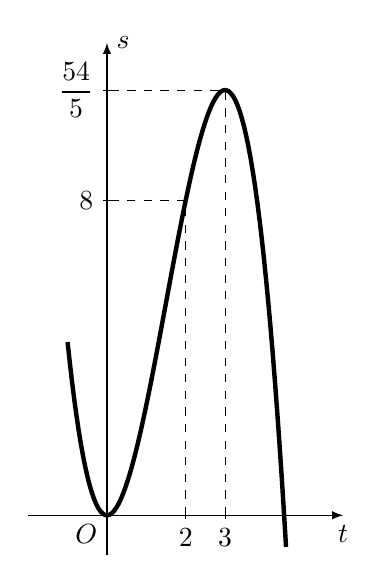
\begin{tikzpicture}[>=latex, scale=0.5]
    % Vẽ hệ trục
    \draw[->] (-2,0) -- (6,0) node[below] {$t$};
    \draw[->] (0,-1) -- (0,12) node[right] {$s$};
    \node[below left] at (0,0) {$O$};
    
    % Đánh dấu các mốc
    \draw (2,0.1) -- (2,-0.1) node[below] {$2$};
    \draw (3,0.1) -- (3,-0.1) node[below] {$3$};
    \draw (0.1,54/5) -- (-0.1,54/5) node[left] {$\dfrac{54}{5}$};
    \draw (0.1,8)--(-0.1,8) node[left] {$8$};
    % Vẽ đồ thị hàm số bậc 3
    \draw[ultra thick, samples=100, domain=-1:4.55] 
       plot (\x, {-4/5*\x*\x*\x + 18/5*\x*\x});
    
    \draw[dashed] (2,0) -- (2,8) -- (0,8);
    \draw[dashed] (3,0) -- (3,54/5) -- (0,54/5);
    
\end{tikzpicture}
\end{center}}

% --- CÂU 13 ---
\questionShortAnswer{0}{4}{Một máy bay trình diễn có đường bay gắn với hệ trục \( Oxy \) được mô phỏng như hình vẽ, trục \( Ox \) gắn với mặt đất. Đường bay có dạng là một phần của đồ thị hàm số phân thức bậc hai trên bậc nhất \( y = f(x) \) có đường tiệm cận đứng là \( x = 2 \). \( G \) là giao điểm của đường tiệm cận xiên của đồ thị hàm số \( y = f(x) \) và trục \( Ox \) được gọi là điểm giới hạn. Biết rằng máy bay xuất phát tại vị trí \( A \) cách gốc tọa độ \( O \) một khoảng 2,5 đơn vị và máy bay khi ở vị trí cao nhất cách điểm xuất phát 1,5 đơn vị theo phương song song với trục \( Ox \) và cách mặt đất 4,5 đơn vị. Vị trí máy bay tiếp đất cách điểm giới hạn một khoảng bằng bao nhiêu?

\begin{center}
\begin{tikzpicture}[>=latex, scale=0.8]
    % Vẽ hệ trục
    \draw[->] (-3,0) -- (12,0) node[below] {$x$};
    \draw[->] (0,-1) -- (0,6) node[right] {$y$};
    \node[below left] at (0,0) {$O$};
    
    % Đánh dấu các mốc
    \draw (2,0.1) -- (2,-0.1) node[below left] {$2$};
    
    % Vẽ đồ thị hàm số
    \draw[thick, samples=100, domain=2.44:10.8] 
        plot (\x, {(-2*\x*\x + 25*\x - 50)/(2*\x - 4)});
    \draw[dashed, samples=100, domain=3:11.2] 
        plot (\x, {-\x + 10.5});
    % Đường tiệm cận
    \draw[dashed] (2,-1) -- (2,6) ;
    
    
    % Điểm A, G
    \fill (2.5,0) circle (3pt) node[above right] {$A$};
    \fill (4,4.5) circle (3pt) node[above] {$B$};
    \fill (10.5,0) circle (3pt) node[above] {$G$};
\end{tikzpicture}
\end{center}}

\end{document}
